% !TEX root = ../my-thesis.tex
%
%\selectlanguage{english}  
\chapter{Land-use legacies and climate change as a double challenge to oak forest resilience: mismatches of geographical and ecological rear edges}\label{sec:dendro}

\newpage

\paragraph{Abstract} \mbox{} \\
Global change challenges ecosystems in xeric locations transformed by intensive human use. Resilience to drought of relict Mediterranean \emph{Quercus pyrenaica} populations in the southern Iberian Peninsula was analyzed in relation to historical records of land use, combining dendroecological growth of adult trees and greenness (EVI) as proxies for secondary and primary growth. The growth trends reflected a strong influence of old land-use legacies (\emph{e.g}. firewood removal) in the current forest structure. Trees were highly sensitive to moisture availability, but both primary growth and secondary growth expressed high resilience to drought events over the short and the long term. Resilience and the tree growth response to climate followed a water-stress gradient. A positive growth trend since the late 1970s was particularly evident in mesic (colder and wetter) high-elevation stands, but absent in the most xeric (warmer and drier) stands. The high values of resilience observed suggest that the studied \emph{Q. pyrenaica} populations are located in a geographical but not a climatic or ecological rear edge. Resilience of oak stands to drought events was not spatially homogeneous across the mountain range, due to differences in ecological conditions and/or past management legacies. This is particularly relevant for rear-edge populations where topographic and biophysical variability can facilitate the existence of refugia.

\newpage

\section{Introduction}\label{sec:dendro:Intro}

The response of species to changing environments (\emph{e.g.} distributional shifts) can be determined largely by population responses at range margins \autocite{HampePetit2005ConservingBiodiversity}. Peripheral populations are usually considered more vulnerable compared with populations at the center of a species' range {[}\emph{i.e.} center-periphery hypothesis; \textcite{SagarinGaines2002AbundantCentre}; \textcite{Pirononetal2017GeographicVariation}{]}. Geographically marginal populations have often been assumed to represent ecologically marginal populations. This means lower performance, higher vulnerability, and thus higher risk of extinction than for populations at the core of the species' range \autocite{Rehmetal2015LosingYour,Pirononetal2017GeographicVariation,VilaCabreraetal2019RefiningPredictions}. Nonetheless, recent reviews report that species- and population-specific responses do not always support this hypothesis \autocite{Sextonetal2009EvolutionEcology,Abelietal2014EffectsMarginality,Oldfatheretal2020RangeEdges}. This is partly because a rear-edge is a multidimensional concept including an ecological (\emph{i.e.} climatic and edaphic), a geographical, and a genetic component \autocite{VilaCabreraetal2019RefiningPredictions}, but also an anthropogenic dimension (\emph{i.e.} land-use). In this respect, to fully understand changes in distribution and abundance of species as a consequence of global change, it is crucial to identify and understand mismatches between the geographical and the ecological rear edges \autocite{VilaCabreraJump2019GreaterGrowth}.

Limits of species distribution are strongly determined by climatic factors and biotic interactions \autocite{Gaston2009GeographicRange,Sextonetal2009EvolutionEcology}. Climate change is expected to cause major shifts in the distribution and abundance of plant communities, and signs already indicate that more intense and longer droughts are altering forest dynamics \autocite{Allenetal2010GlobalOverview}. Drought frequency and severity have increased in recent decades, with a trend towards drier summers, particularly for Southern Europe \autocite{VicenteSerranoetal2014EvidenceIncreasing,Staggeetal2017ObservedDrought}. In this climatic-change context, population loss and range retractions are expected in boreal, temperate, and Mediterranean species at the lowest latitudes and elevations, as well as in drought-prone areas of a species' distribution, \emph{i.e.} the rear edge. The rear-edge populations are likely to be more sensitive to minor climatic and microtopographic variations and therefore the effects of droughts are expected to be particularly noteworthy \autocite{HampePetit2005ConservingBiodiversity,VilaCabreraetal2019RefiningPredictions}.

It is often overlooked that human activity constitutes a driver of change as powerful or even more powerful as natural drivers, \emph{i.e.} natural variation in climate, particularly for regions with long land-use history such as the Mediterranean Region \autocites[\emph{e.g.}][]{NavarroGonzalezetal2013WeightLanduse,DoblasMirandaetal2017ReviewCombination}. In these areas, the susceptibility and response of ecosystems to climate change are conditioned by legacies of historical land-use activity \autocites[\emph{e.g.}][]{Munteanuetal2015Legacies19th,Mausolfetal2018LegacyEffects}. The past land-use legacies interact with recent human-caused climate disturbances and may confound their interpretation \autocite{Fosteretal2003ImportanceLanduse}. For example, recent works showed that a quarter of current forests in the Iberian Peninsula, are growing on former agricultural and grazing land abandoned after the 1950s \autocite{VilaCabreraetal2017NewForests}. Consequently, anthropogenic habitat modification and its legacies represent a critical dimension of marginality as they may intensify, confound or delay climate-driven population decline at rear edges \autocite{VilaCabreraJump2019GreaterGrowth,SanchezdeDiosetal2020FagusSylvatica}. In this context, our work seeks to identify the impacts and responses to natural (\emph{e.g.} severe drought) and human disturbances (\emph{e.g.} logging) on oak forests at their southern geographical range. A historical perspective should help us to interpret the responses of ecosystems to disturbances \autocite{Fosteretal2003ImportanceLanduse}, particularly regarding marginal rear-edge populations \autocite{VilaCabreraetal2019RefiningPredictions}.

The assessment of resilience to climate and human disturbances provides critical information concerning the capacity of forests to maintain their structure and render valuable ecosystem services. Resilience is the capacity of an ecosystem to persist and maintain its state and functions in the face of disturbance \autocite{Holling1973ResilienceStability,Hodgsonetal2015WhatYou}. \textcite{Lloretetal2011ComponentsTree} proposed an approach, which decomposes resilience into three components: resistance to drought, recovery after drought and resilience. This resilience is determined by the forest's ability to mitigate the disturbance (resistance) and the capacity to recover from the impact (recovery) \autocite{IngrischBahn2018ComparableQuantification}. This conceptual approach has recently become widely used to assess forest resilience, because it allows a simple, yet highly efficient assessment of short-term responses of trees to drought. Nevertheless, not exempt from criticism, this approach needs to be applied carefully to avoid potential bias at different levels \autocite{Schwarzetal2020QuantifyingGrowth}. In this sense we assessed forest resilience both over the short-term to several recent extreme drought episodes, as well as over the long-term to climate change (\emph{i.e.} warming on the last few decades), using two different proxies to characterize resilience. Dendroecological estimates of growth (\emph{i.e.} tree-ring width) are commonly used proxies to characterize tree vitality and have commonly been used to study growth changes in response to drought at the individual tree level \autocite{Fritts1976TreeRings,Dobbertin2005TreeGrowth}. Remote sensing can be used to analyze the impact of drought on ecosystems at the stand level \autocite[\emph{e.g.}][]{Zhangetal2013MonitoringEstimating}. Tree-ring records complement remote-sensing data with a longer time scale. Tree rings can reflect tree-growth anomalies induced by climate or other disturbance over decades to centuries \autocite{Babstetal2017ImprovedTreering} and provide an accurate measure of growth responses to droughts \autocite{Bhuyanetal2017DifferentResponses}. The combination of remote sensing and dendroecology has been used to assess the effects of droughts on vegetation along ecological gradients \autocites[\emph{e.g.}][]{VicenteSerranoetal2013ResponseVegetation,Coulthardetal2017TreeGrowth}, and also to evaluate growth resilience to drought in several tree species \autocites[\emph{e.g.}][]{Gazoletal2018ForestResilience,PenaGallardoetal2018DroughtSensitiveness}.

In the present study, we assess resilience of \emph{Quercus pyrenaica} Willd. (Pyrenean oak) from southern relict forests at the rear edge of the species distribution, where species performance is considered to be threatened by climate change \autocite{GeaIzquierdoetal2013GrowthProjections,GeaIzquierdoetal2017RiskyFuture}. For this, we combined remote-sensing information and dendroecological methods to evaluate the impact of drought both on canopy greenness (as a proxy for primary growth) and radial tree growth (as a proxy for secondary growth). For the analysis of forest resilience to climate, we took into account the land-use history of these transformed forests, thoroughly reviewing historical documents to reconstruct forest history at the study sites, and analyzing how anthropogenic drivers have shaped the current forest structure. Based on this analysis, we developed a rationale that integrates the ecological and anthropogenic components of marginality to determine the regional and local scale mechanisms shaping the probability of persistence (or extinction) of rear-edge oak populations. Our main hypothesis is that range edge stands will show low resilience to extreme droughts, but that the vulnerability to drought will be reduced quickly across a fine-scale topographic gradient of decreasing aridity. To test this hypothesis, we: (\emph{i}) quantified how recent extreme drought events influenced primary and secondary growth of \emph{Q. pyrenaica} forests at their present geographical rear edge; (\emph{ii}) analyzed the long-term resilience of these forests to extreme drought events, using time-series of radial growth; (\emph{iii}) reviewed historical documents to reconstruct forest-management history and to infer how it impacted tree growth and stand dynamics over time; (\emph{iv}) and examined differences in the resilience metrics between populations under contrasting ecological conditions (\emph{i.e.} xeric \emph{vs.} mesic) along environmental gradients within the rear edge in order to detect vulnerability to climate change at the small spatial scale.

\begin{sidewaystable} 
\caption{Characteristics of sampled plot. Lat = latitude; Long = longitude. Dbh and height of all trees, Basal Area (BA), Density and SRD (size ratio proportional to distance) are computed for all trees within a 10-m radius of focal trees (see Materials and methods). Temp.: annual average of mean monthly minimum and maximum temperatures. Values shown here correspond to site averages. Standard deviations are shown in parentheses. Different letters indicate statistically significant differences between sites (Kruskal-Wallis test followed by Dunn’s test, \emph{p<0.05}). Stands were monospecific, hence all results correspond to oak data.}\label{tab:sampledPlots}
\begin{adjustbox}{width=\linewidth}
\begin{threeparttable}
\begin{tabular}{p{1cm}p{1.2cm}p{1.2cm}p{2.3cm}p{1.3cm}p{1cm}p{1.3cm}p{2cm}p{1.4cm}p{1.3cm}p{1.6cm}p{1.8cm}p{1.8cm}p{1.9cm}p{2cm}p{1.8cm}}
 &  &  &  &  &  &  & \multicolumn{4}{l}{Cored trees} & \multicolumn{5}{l}{Stand competition} \\ \cline{8-16}
\textbf{Site} & \textbf{Lat (º)} & \textbf{Long (º)} & \textbf{Elevation (m)} & \textbf{Slope (º)} & \textbf{Prec. (mm)} & \textbf{Temp. (ºC)} & \textbf{\#trees (\#cores)} & \textbf{Dbh (cm)} & \textbf{Height (m)} & \textbf{Age (years)} & \textbf{Dbh all (cm)} & \textbf{Height all (m)} & \textbf{BA (m\textsuperscript{2}ha\textsuperscript{-1})} & \textbf{Density (trees ha\textsuperscript{-1})} & \textbf{SDR} \\ \hline
CA-High & 36.97 & -3.42 & 1846 - 1884 & 12.11 (3.28) & 731 & 3.4-13.8 & 15 (30) & 69.8 (20.5) a & 15.4 (1.8) a & 161.0 (32.2) a & 34.1 (24.3) a & 10.8 (4.4) a & 39.13 (24.31) a & 348.0 (147.1) a & 0.91 (0.63) a \\
CA-Low & 36.96 & -3.42 & 1691 - 1751 & 12.86 (2.98) & 658 & 4.7-15.6 & 15 (30) & 45.9 (8.6) a & 12.6 (1.6) b & 148.5 (16.5) a & 21.7 (14.4) b & 9.0 (2.8) b & 18.02 (7.11) ab & 409.6 (226.0) a & 0.89 (0.44) a \\
SJ & 37.13 & -3.37 & 1322 - 1474 & 27.33 (5.59) & 555 & 4.9-16.35 & 20 (48) & 31.9 (3.7) b & 11.8 (2.3) b & 72.6 (11.1) b & 20.6 (8.1) b & 9.7 (3.6) ab & 11.64 (5.47) b & 339.0 (130.3) a & 1.11 (0.52) a \\ \hline
\end{tabular}%
\end{threeparttable}
\end{adjustbox}
\end{sidewaystable}

\section{Material and Methods}\label{sec:dendro:MatMet}
\subsection{Tree species and study site}\label{sec:dendro:StudyArea}
\emph{Quercus pyrenaica} forests extend throughout south-western France and the Iberian Peninsula, reaching their southern limit in mountain areas of northern Morocco \autocite{Franco1990Quercus}. In the Iberian Peninsula, these forests occupy siliceous soils under meso-supramediterranean and mesotemperate areas and subhumid, humid, and hyperhumid ombroclimate. Pyrenean oak is a deciduous species that requires over 650 mm of annual precipitation and some summer precipitation. As a submediterranean species, it has lower drought tolerance than evergreen Mediterranean taxa \autocite{delRioetal2007BioclimaticAnalysis}.

\begin{figure}
\centering
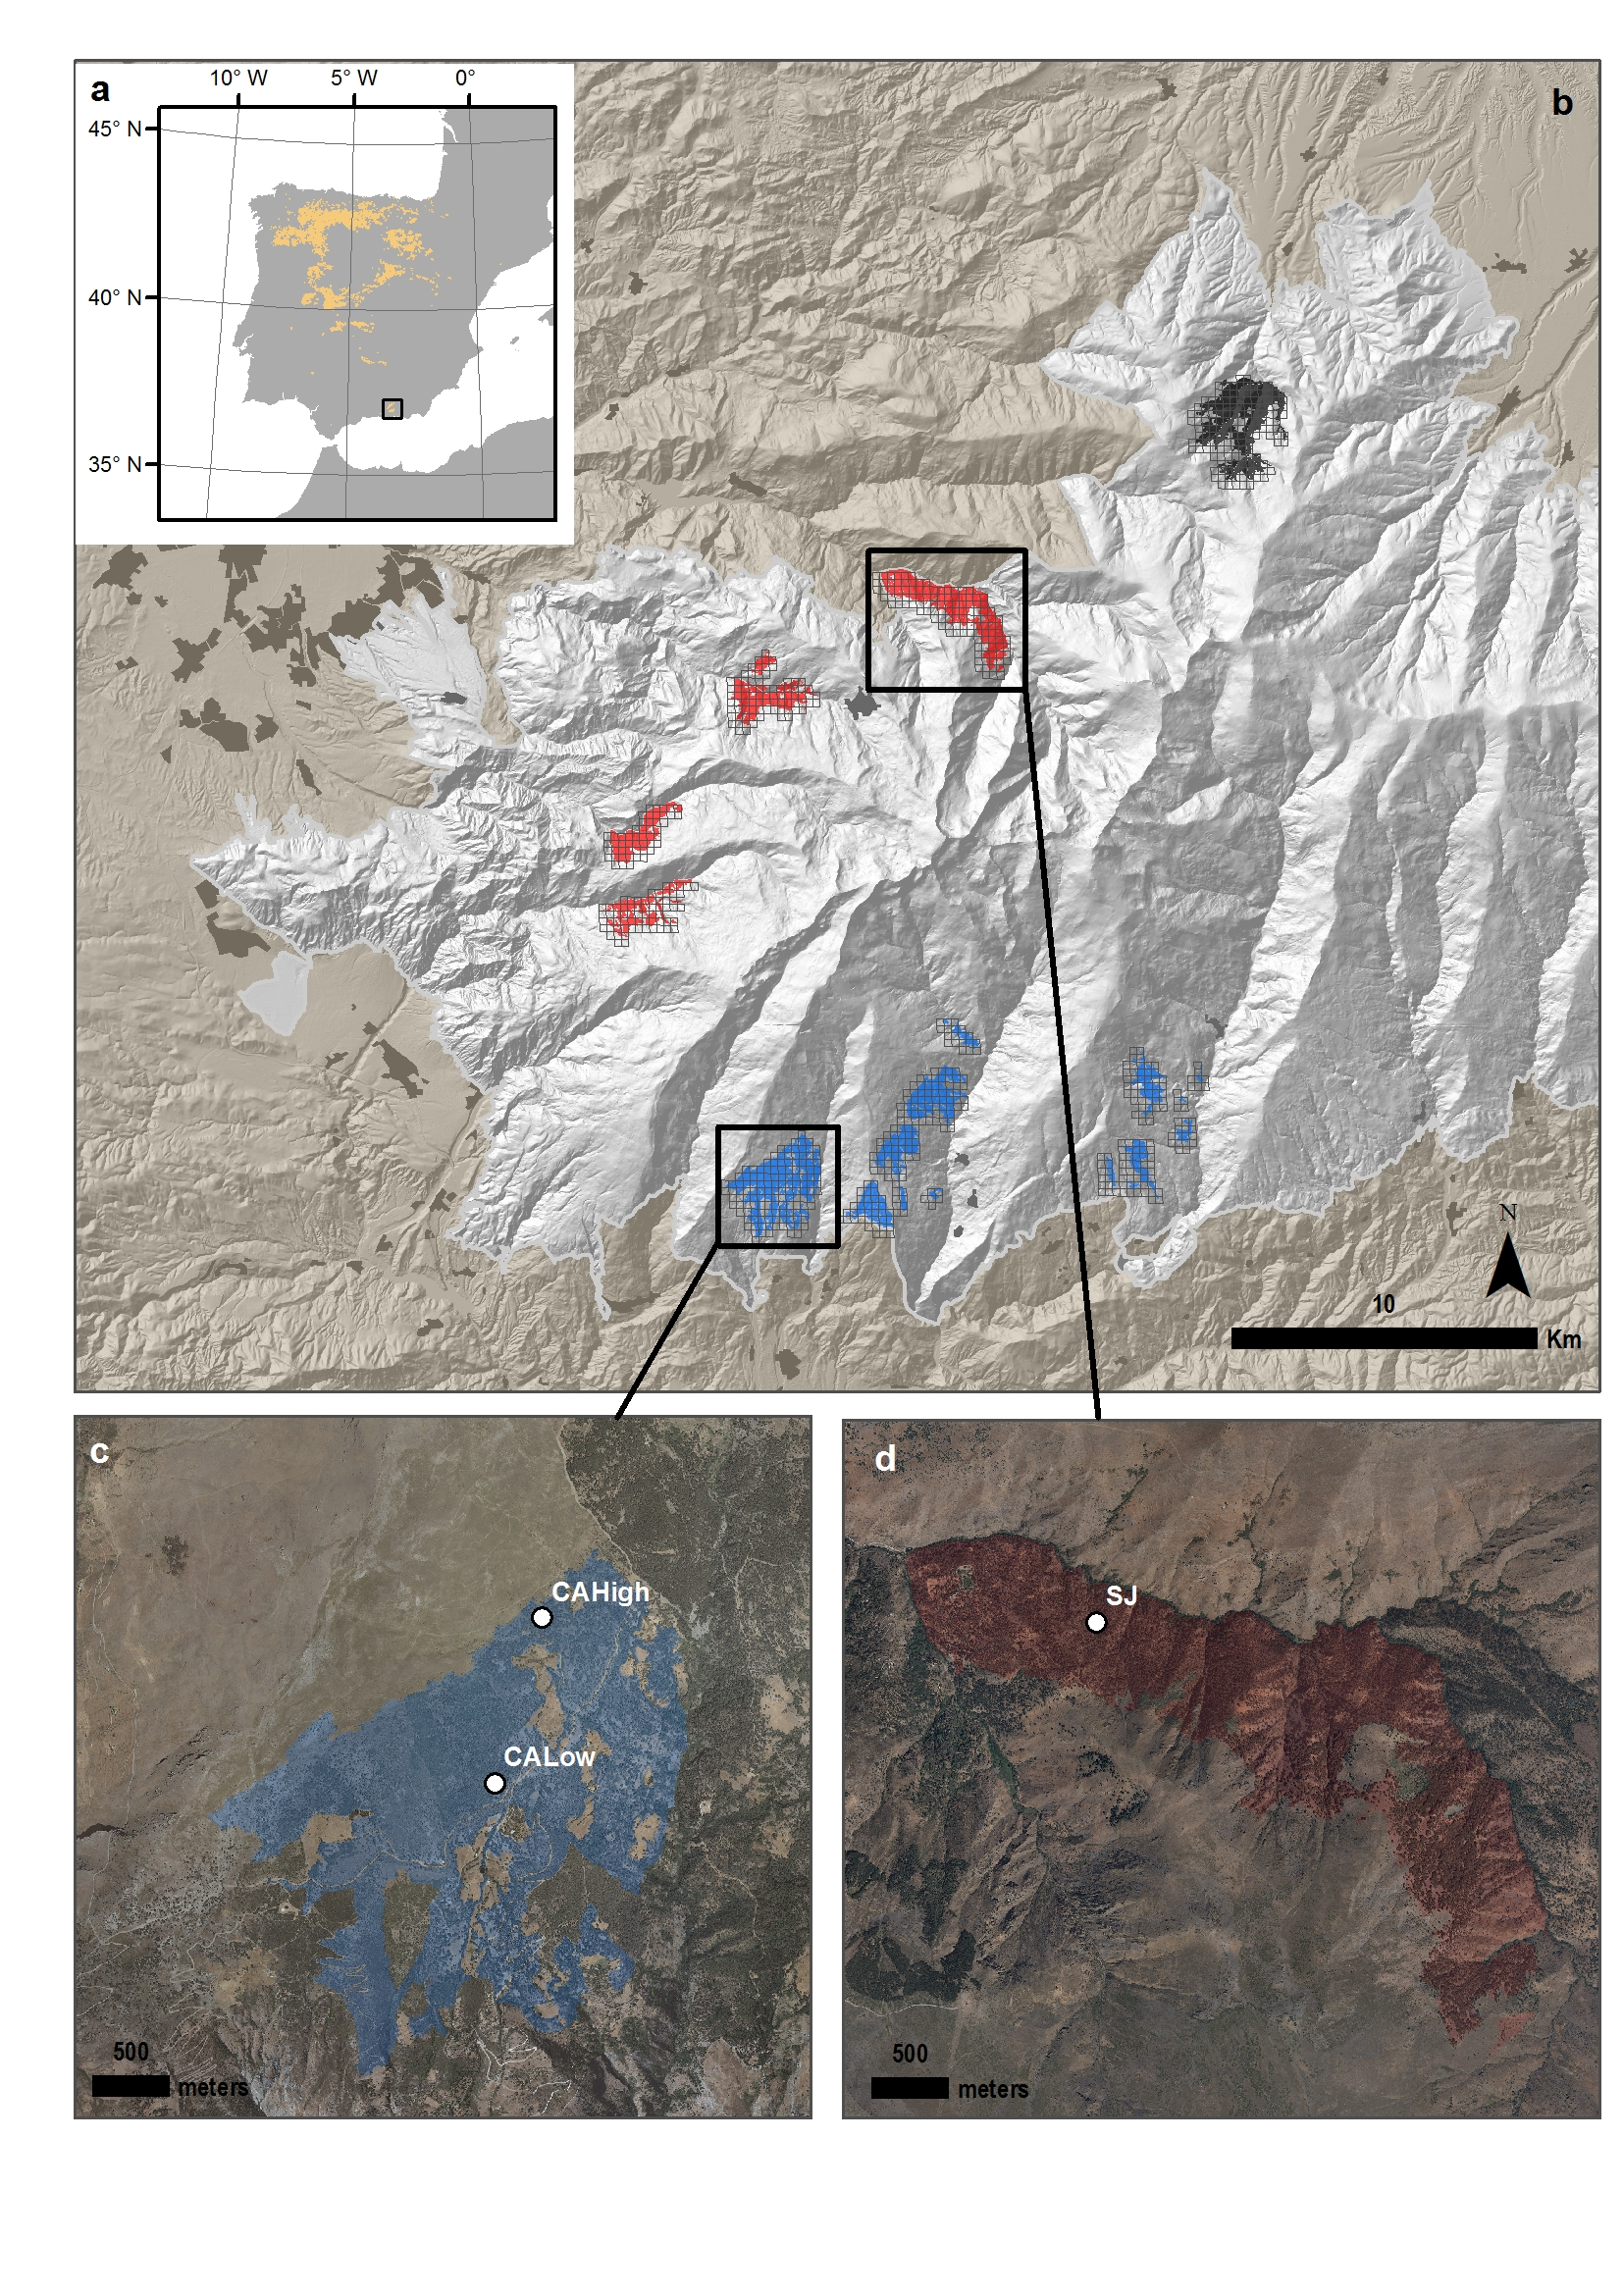
\includegraphics[width=\textwidth]{img/dendro/dendro-mapa.jpg} \caption{Distribution of \textit{Quercus pyrenaica} forests in the Iberian Peninsula \textbf{a} and in Sierra Nevada mountain range \textbf{b}. Different colors indicate oak-population clusters identified in Sierra Nevada \autocite{PerezLuque2015}. For each population, a grid with the MODIS pixels is shown (see Material and methods). Detailed location of the dendroecological sampling sites: northern (San Juan, SJ) \textbf{c}, and southern ones (Cáñar: CA-Low and CA-High) \textbf{d}. Color orthophotography of 2009 from Regional Ministry of the Environment.}
\label{fig:map}
\end{figure}

The forests of this species reach their southernmost European limit in Andalusian mountains such as Sierra Nevada (37°N, 3°W), a high-mountain range with elevations of up to 3482 m \emph{a.s.l.}. The climate is Mediterranean, characterized by cold winters and hot summers, with pronounced summer drought and increasing aridity with decreasing altitude, and marked variability in annual rainfall according to elevation and aspect. Sierra Nevada is considered a glacial refuge for deciduous \emph{Quercus} species \autocite{Olaldeetal2002WhiteOaks}. Eight Pyrenean oak patches (2400 ha) have been identified in this mountain range (\figref{fig:map}), from 1100 to 2000 m \emph{a.s.l.} and often associated with major river valleys. Today, \emph{Quercus pyrenaica} woodlands in this mountain region represent a rear edge of their habitat distribution \autocite{HampePetit2005ConservingBiodiversity}. They are the richest forest formation in vascular plant species of Sierra Nevada, containing several endemic and endangered plant species \autocite{Loriteetal2008PhytosociologicalReview}. They also harbor high levels of intraspecific genetic diversity \autocite{ValbuenaCarabanaGil2013GeneticResilience}. These relict forests have undergone intensive human use throughout history \autocite{CamachoOlmedoetal2002DinamicaEvolutiva}. Furthermore, the conservation status of this species for southern Spain is considered ``Vulnerable'' and it is expected to suffer from climate change, potentially reducing its suitable habitats in the near future \autocite{GeaIzquierdoetal2013GrowthProjections,GeaIzquierdoetal2017RiskyFuture}.
